\newcommand{\nrandom}{\num{700}}
\newcommand{\napplication}{\num{60}}
\newcommand{\nstrategic}{\num{60}}

\section{Evaluation}
\label{sect:ressat-evaluation}

We evaluated the proposed~\cref{alg:ressat} against
the state-of-the-art DPLL-based SSAT solver \dcssat~\cite{Majercik2005}
over three families of random-exist quantified SSAT formulas.
The proposed algorithm is implemented in the \texttt{C++} language inside the \abc~\cite{ABC} environment.
The SAT solver \minisat-2.2~\cite{Een2003Solver}
and the model counter \cachet~\cite{Sang2004}
are used as underlying computational engines.
Our prototyping implementation\footnote{Available at: \url{\ssatabcurl}} is named \ressat.
A bare version of \ressat without minterm generalization is called \ressatb in the experiments.
We used \ssatABCRevision for the evaluation.
The solver \dcssat,
which is also implemented in the \texttt{C++} language,
was kindly provided by its author Majercik.

\subsection{Benchmark set}
Three sets of random-exist quantified SSAT formulas\footnote{Available at: \url{\ssatbenchmarkurl}},
including random $k$-CNF formulas,
planning formulas,
and probabilistic equivalence checking formulas,
were used in the evaluation.
We used \ssatBenchRevision in the experiments.

\subsubsection{Random $k$-CNF formulas}
The random $k$-CNF formulas are generated using the CNF generator \cnfgen~\cite{Lauria2017CNFgen}.
Let $k$ be the number of literals in a clause,
$n$ be the number of variables of a formula,
and $m$ be the number of clauses of a formula.
The CNF formulas were generated with the following parameter settings.
Let $k$ range from 3 to 9,
$n$ equal 10, 20, 30, 40, and 50,
and the clauses-to-variables ratio $\frac{m}{n}$ range from $k-1$ to $k+2$.
For each combination of parameters,
five formulas were sampled.
As a result,~\nrandom~CNF formulas were generated.
To convert the generated formulas to random-exist quantified SSAT formulas,
half of the variables in a formula are randomly quantified with probability $0.5$,
and the rest of the variables are existentially quantified.

\subsubsection{Planning formulas}
We use the \textit{strategic-company} problem~\cite{Cadoli1997} as an example
to evaluate the performance of the SSAT solvers over planning formulas.
We briefly describe the problem as follows.
Suppose a businessman owns $n$ companies that produce $m$ different kinds of products.
A company is \textit{strategic} if it is in a minimal set of companies that together produce all kinds of products.
The information about a company being strategic is valuable to the businessman.
Suppose the businessman considers selling out some companies upon a financial crisis,
but still hopes to produce every kind of products.
The businessman would prefer selling out a non-strategic company.
The problem becomes more complicated if the \textit{controlling relations} are taken into account.
If a company is \textit{controlled} by some other companies,
the company can be sold out only if some of its controlling companies is also sold out.
The problem to decide whether a company is strategic can be encoded as a forall-exist quantified QBF~\cite{Faber2005,Leone2006}.

We modify the QBFs encoding the strategic-company problem
to their SSAT variants by replacing the universal quantifiers in the original QBFs
with randomized ones with probabilities $0.5$.
These QBFs are taken from \texttt{QBFLIB}~\cite{Narizzano2006}.
The satisfying probability reflects the likelihood for a company to be strategic.
The QBFs that we experimented with have the following parameter settings:
$n$ equals 5, 10, 15, $\ldots$, 75, $m=3n$,
and the number of controlling relations equals 4, 9, 14, and 19.
In total, there are~\nstrategic~strategic-company formulas.

\subsection{Experimental setup}
Our experiments were performed on a machine with~\machineSpec.
The operating system was~\osInfo.
The programs were compiled with~\compiler.
Each SSAT-solving task was limited to a CPU core,
a CPU time of~\timelimit,
and a memory usage of~\memlimit.
To achieve reliable benchmarking,
we used a benchmarking framework \benchexec\footnote{Available at: \url{\benchexecurl}}~\cite{Benchmarking-STTT}.

\subsection{Results}

\subsubsection{Random $k$-CNF formulas}

\begin{figure*}[hp]
    \centering
    \subfloat[CPU time]{
        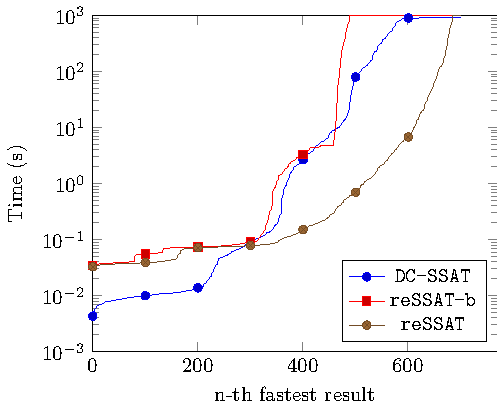
\includegraphics{random-exist-ssat/evaluation/plots/quantile-cputime-Random.pdf}
        \label{fig:ressat-quantile-cputime-random}
    }\\
    \subfloat[Memory usage]{
        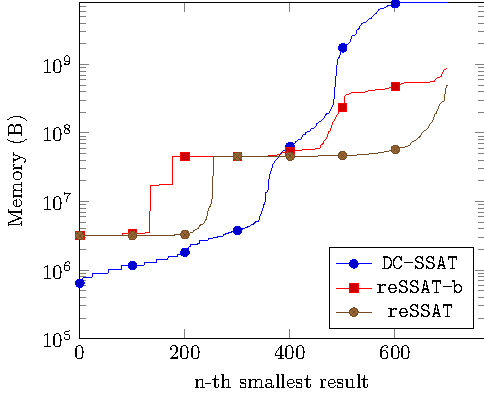
\includegraphics{random-exist-ssat/evaluation/plots/quantile-memory-Random.pdf}
        \label{fig:ressat-quantile-memory-random}
    }
    \caption{Quantile plots of random $k$-CNF formulas}
    \label{fig:ressat-quantile-random}
\end{figure*}

\Cref{fig:ressat-quantile-random} shows the quantile plots regarding CPU time and memory usage
of the SSAT instances derived from the random $k$-CNF formulas.
A data point $(x,y)$ in a quantile plot indicates that
there are $x$ formulas processed by the respective algorithm within a resource constraint of $y$.
In~\cref{fig:ressat-quantile-cputime-random},
we observe that \ressat not only solved more formulas than \dcssat,
but was also more efficient.
Moreover, the minterm-generalization technique is crucial for the performance of \ressat,
as can be seen from the huge gap between \ressat and \ressatb.
On the other hand,
\cref{fig:ressat-quantile-memory-random} shows that the memory usage of \dcssat is about two orders of magnitude greater than that of \ressat for large formulas.
This can be attributed to the subformula caching of \dcssat.
Instead, \ressat stores information as SAT or UNSAT cubes,
which are more compact than subformulas.

\subsubsection{Strategic-company formulas}

\begin{figure*}[t]
    \centering
    \subfloat[CPU time]{
        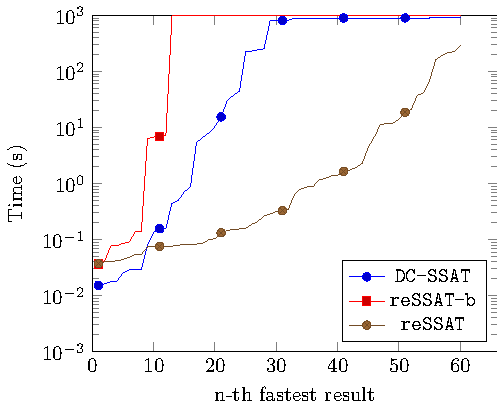
\includegraphics{random-exist-ssat/evaluation/plots/quantile-cputime-Strategic.pdf}
        \label{fig:ressat-quantile-cputime-strategic}
    }\\
    \subfloat[Memory usage]{
        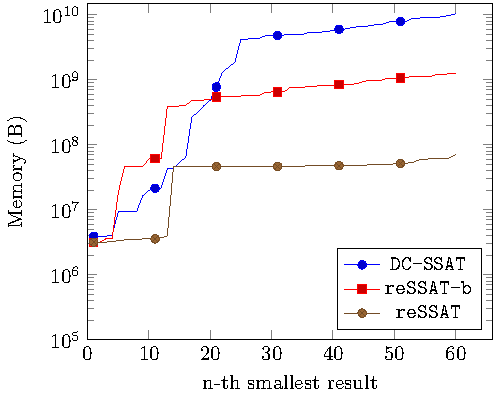
\includegraphics{random-exist-ssat/evaluation/plots/quantile-memory-Strategic.pdf}
        \label{fig:ressat-quantile-memory-strategic}
    }
    \caption{Quantile plots of strategic-company formulas}
    \label{fig:ressat-quantile-strategic}
\end{figure*}

\Cref{fig:ressat-quantile-strategic} shows the quantile plots of the SSAT instances
derived from the strategic-company formulas.
The results are similar to those of random $k$-CNF formulas,
showing that \ressat also works well on structured instances from AI applications.
Compared to \dcssat,
\ressat was able to solve all strategic-company formulas with much smaller memory usage.
The performance gap between \ressat and \ressatb again confirms the importance of the minterm-generalization technique.

\subsubsection{Probabilistic equivalence checking formulas}

\begin{table}[hp]
    \centering
    \scriptsize
    \caption{Results of solving PEC formulas ($\dr=0.01$)}
    \label{tbl:random-exist-ssat-pec-0.01}
    \pgfplotstabletypeset[
        every head row/.style={before row={\toprule
                        & \multicolumn{4}{c}{\dcssat} & \multicolumn{6}{c}{\ressat} & \multicolumn{6}{c}{\ressatb}\\},after row=\midrule},
        every last row/.style={after row=\bottomrule},
        empty cells with={--},
        formula column/.list={0},
        time column/.list={1,3,6},
        prob column/.list={2,4,7},
        ubound column/.list={5,8}
    ]
    {random-exist-ssat/evaluation/csv/parsed-PEC-0.01.csv}
\end{table}

\begin{table}[hp]
    \centering
    \scriptsize
    \caption{Results of solving PEC formulas ($\dr=0.1$)}
    \label{tbl:random-exist-ssat-pec-0.10}
    \pgfplotstabletypeset[
        every head row/.style={before row={\toprule
                        & \multicolumn{4}{c}{\dcssat} & \multicolumn{6}{c}{\ressat} & \multicolumn{6}{c}{\ressatb}\\},after row=\midrule},
        every last row/.style={after row=\bottomrule},
        empty cells with={--},
        formula column/.list={0},
        time column/.list={1,3,6},
        prob column/.list={2,4,7},
        ubound column/.list={5,8}
    ]
    {random-exist-ssat/evaluation/csv/parsed-PEC-0.10.csv}
\end{table}
